\vspace{-0.1cm}\section{Evaluation}\label{chap4-sec:eval}

%\ji{1. Run experiments with smaller constants, where an honest user might even be caught. 2. Rerun experiments and show error for just user who was attacked. 3. Rerun experiments with non-random degree deflation attacks.}
In this section, we present our evaluation results. Our evaluation seeks to empirically answer the following questions:
\squishlist
    \item \textbf{Q1.} How do the different protocols perform in terms of correctness and soundness?
   % \item \textbf{Q2.} How effective are the degree inflation and deflation attacks on the algorithms?
    \item \textbf{Q2.} How do the efficacies of input and response poisoning attacks compare?
    \item \textbf{Q3.} What is the impact of the privacy parameter $\epsilon$ on the poisoning attacks?
\squishend
%We answer these questions in the following three sections.
  \vspace{-0.4cm}  \subsection{Experimental Setup}\label{chap4-sec:exp-setup}
\begin{comment}
\begin{enumerate}
    \item threshold reduced to 0.4
    \item Deflation - users' friends are attacked, stronger attack
    \item Inflation - target's error increase, target disqualified
    \item target is always the max for response, sometimes get disqualified ,
\end{enumerate}
High epsilon honest users responses will be true mostly and so, you get disqualified, inflation, 10's disqualified, 11s are degree, assymmtery between deflation/inflation

High epsilon not possible to cheat, because if our design, random noise might be greater than target- inflation

Honest users control your degree

\textbf{TO-DO}
\begin{enumerate}
\item Run stronger input,response for degree inflation -- max is close to target
\item we want some disqualifications but not all - lower threshold honest users never disqualified
\item Fix: Degree deflation FB - input is worse than response
\end{enumerate}
\end{comment}
\noindent\textbf{Datasets.} We evaluate our protocols on two graphs -- a real-world sparse graph and a synthetically generated dense graph.
\squishlist
    \item \textit{FB.} This graph  corresponds to data from Facebook~\cite{FB} representing the friendships of 4082 Facebook users. The graph has $88$K edges. %This simulates running the protocols on a real-world social network.
    \item \textit{Syn.} To test a more dense regime, we evaluate our protocols on a synthetic graph generated using the Erdos-Renyi model~\cite{ER} with parameters $G(n=4000, p=0.5)$ ($n$ is the number of edges; $p$ is the probability of including any edge in the graph).  The graph has $\approx 8$ million edges. %In such dense graphs, the error introduced by randomized response is acceptable as the degrees are $O(n)$, and thus we expect the protocols to perform better for this regime.
\squishend

\begin{figure*}[hbt!]
\begin{subfigure}[b]{\linewidth}
        \centering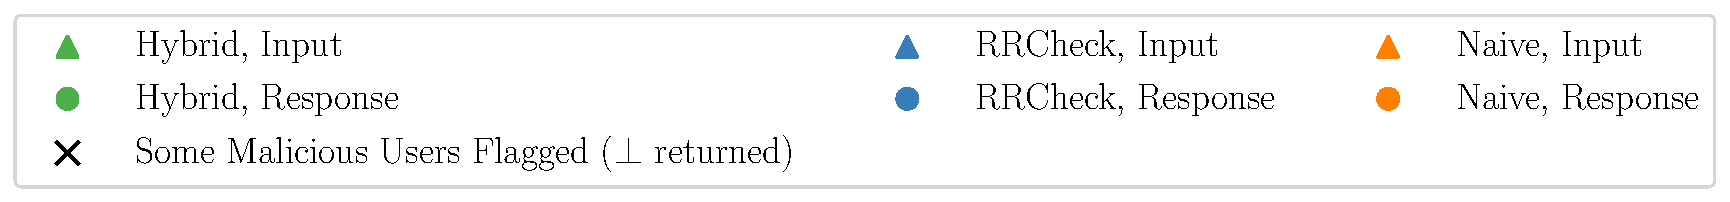
\includegraphics[width=0.8\linewidth]{Plots/legend.pdf}
        \end{subfigure}\\
 \begin{subfigure}[b]{\linewidth}
     
         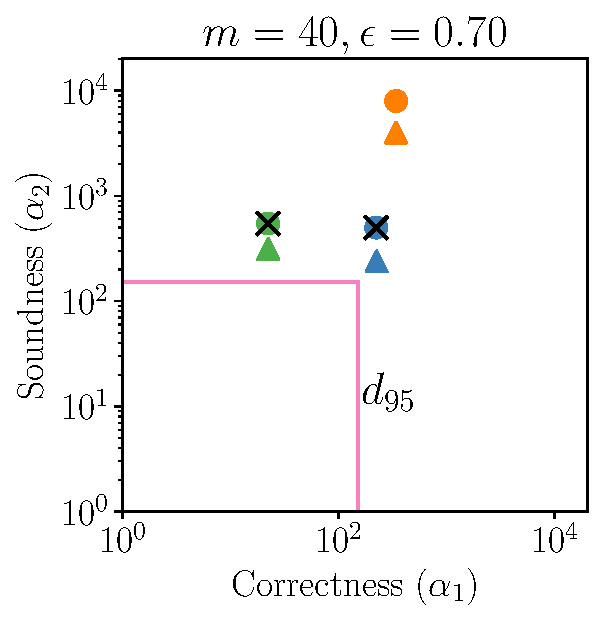
\includegraphics[width=0.23\linewidth]{Plots/fb_inf_40_0.7.pdf}
 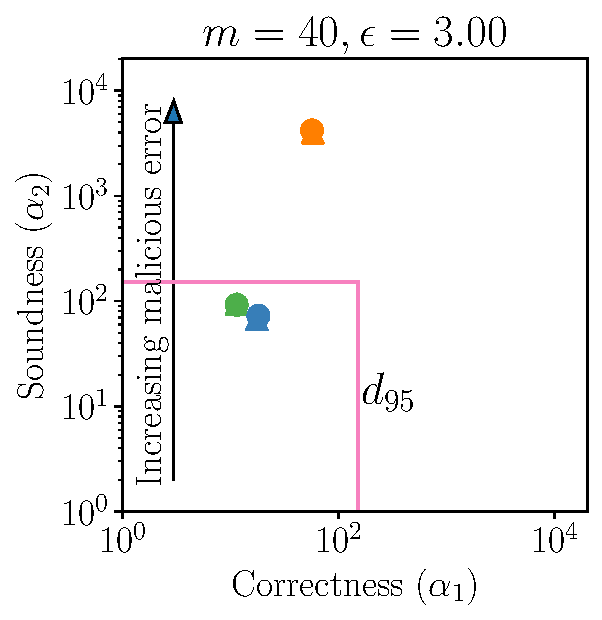
\includegraphics[width=0.23\linewidth]{Plots/fb_inf_40_3.0.pdf}   
  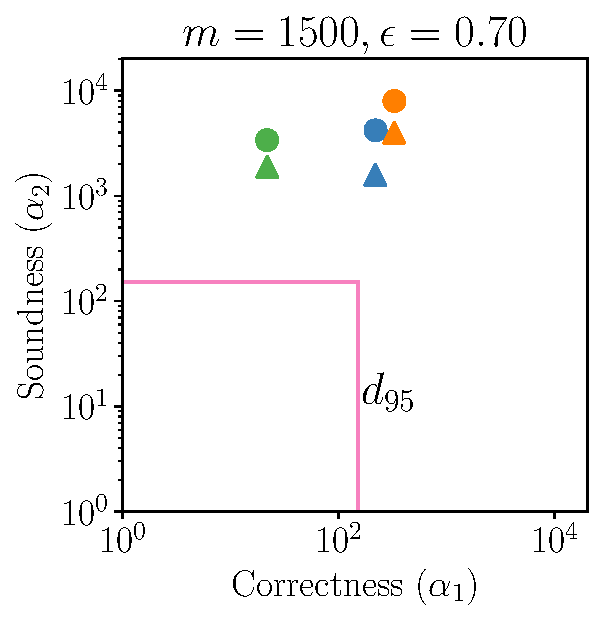
\includegraphics[width=0.23\linewidth]{Plots/fb_inf_1500_0.7.pdf} 
   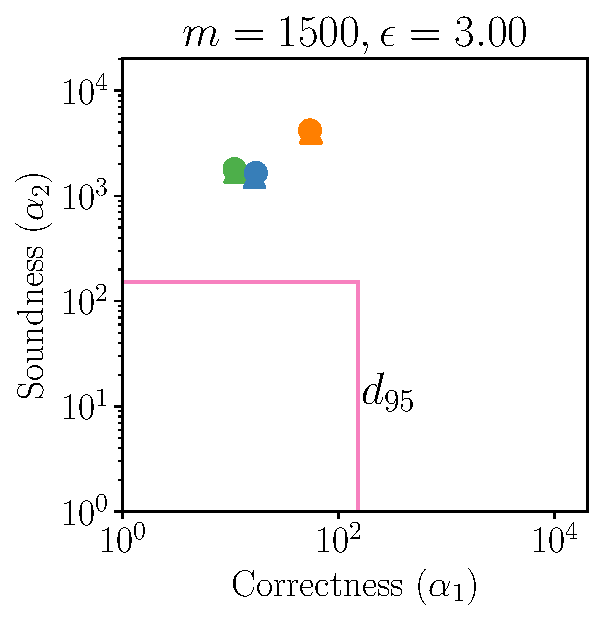
\includegraphics[width=0.23\linewidth]{Plots/fb_inf_1500_3.0.pdf} 
 \caption{\scalebox{0.8}{\textit{FB}: Degree Inflation Attack}}
        \label{chap4-fig:FB:infl}\end{subfigure}%%
    \\
    \begin{subfigure}[b]{\linewidth}
     
         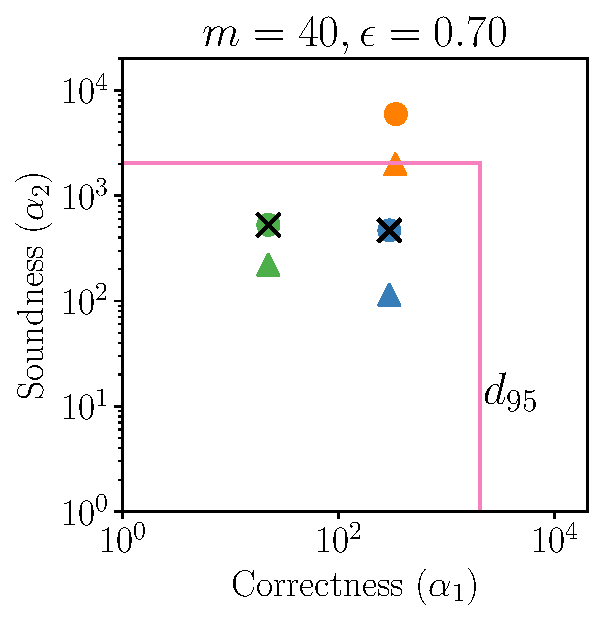
\includegraphics[width=0.23\linewidth]{Plots/gnm_inf_40_0.7.pdf}
 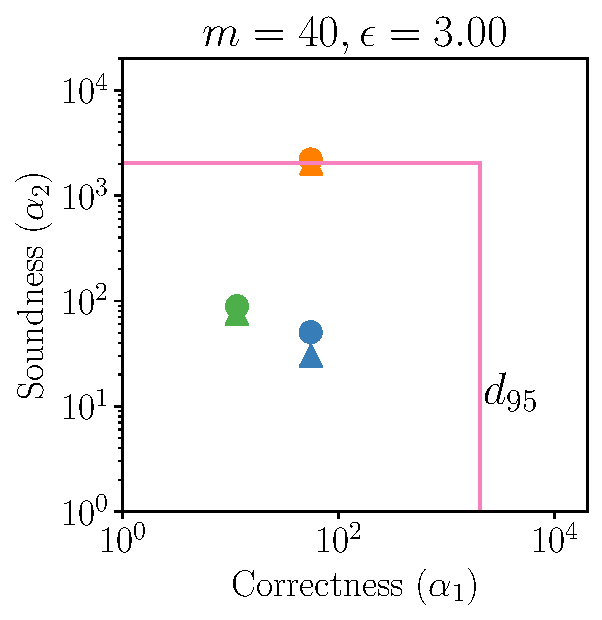
\includegraphics[width=0.23\linewidth]{Plots/gnm_inf_40_3.0.pdf}   
   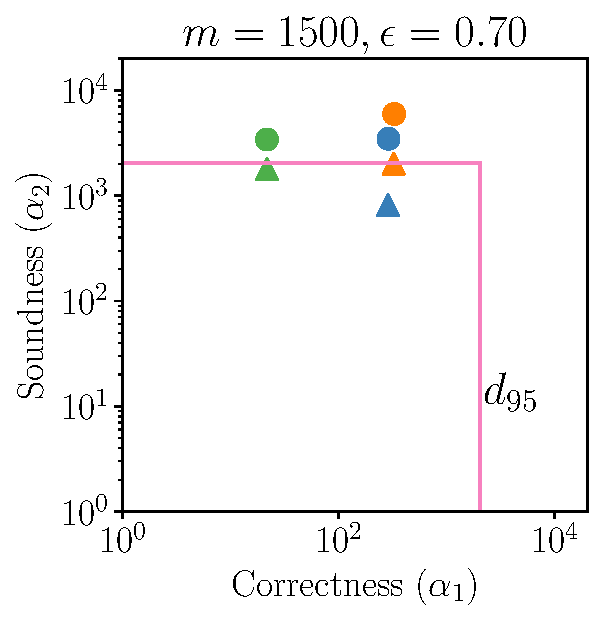
\includegraphics[width=0.23\linewidth]{Plots/gnm_inf_1500_0.7.pdf}
 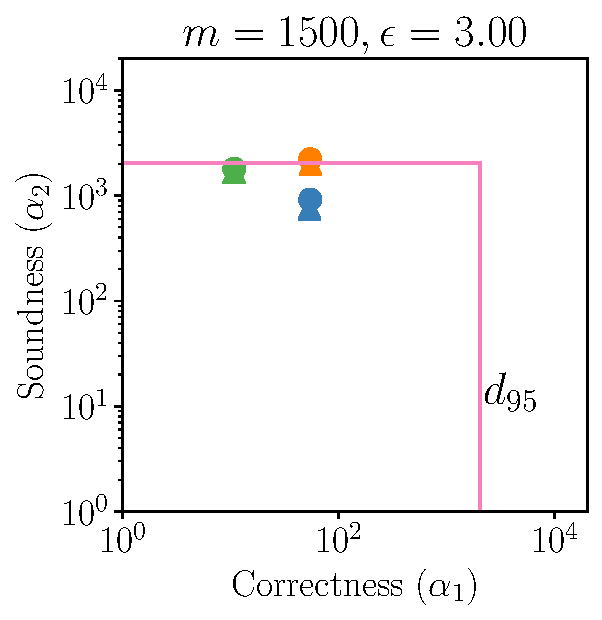
\includegraphics[width=0.23\linewidth]{Plots/gnm_inf_1500_3.0.pdf} 
\caption{\scalebox{0.8}{\textit{Syn}: Degree Inflation Attack}}
        \label{chap4-fig:syn:infl}\end{subfigure}%%
   
  \caption{Robustness Analysis for Degree Inflation Attack: We plot the empirical correctness (error of honest user) and soundness (error of malicious user). $d_{95}$ denotes the $95$-th percentile of the degree distribution.}
   \label{chap4-fig:analysis}%\vspace{-0.5cm}
\end{figure*}

\begin{figure*}[hbt!]
\begin{subfigure}[b]{\linewidth}

    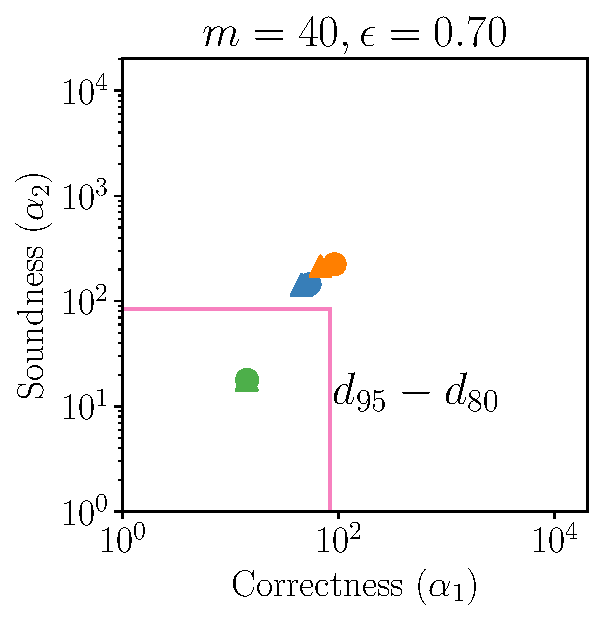
\includegraphics[width=0.23\linewidth]{Plots/fb_def_40_0.7.pdf}
 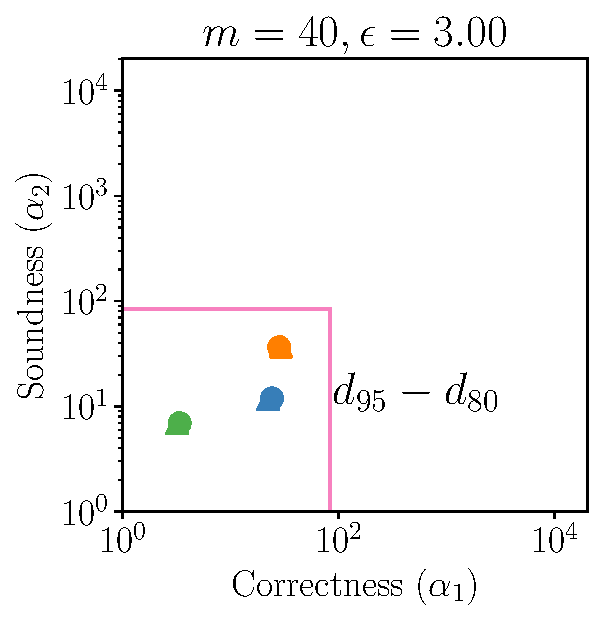
\includegraphics[width=0.23\linewidth]{Plots/fb_def_40_3.0.pdf}
    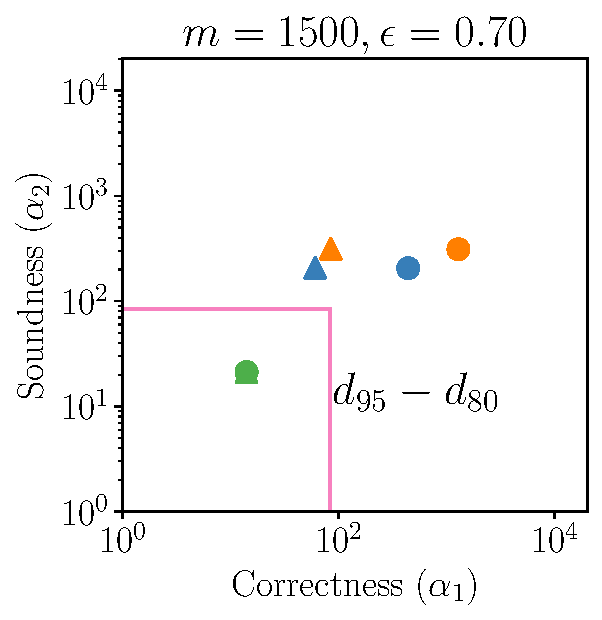
\includegraphics[width=0.23\linewidth]{Plots/fb_def_1500_0.7.pdf}
 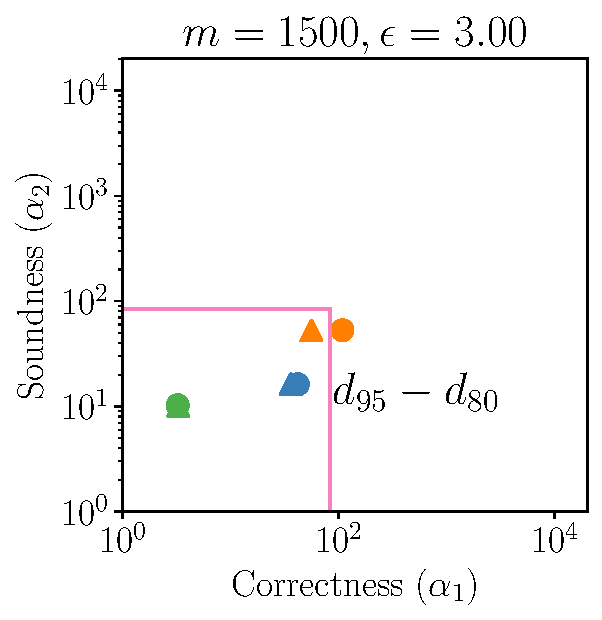
\includegraphics[width=0.23\linewidth]{Plots/fb_def_1500_3.0.pdf}
  \vspace{-0.2cm}  \caption{\scalebox{0.8}{\textit{FB}: Degree Deflation Attack}}
    \label{chap4-fig:FB:defl}
    \end{subfigure}\\
 \begin{subfigure}[b]{1\linewidth}
 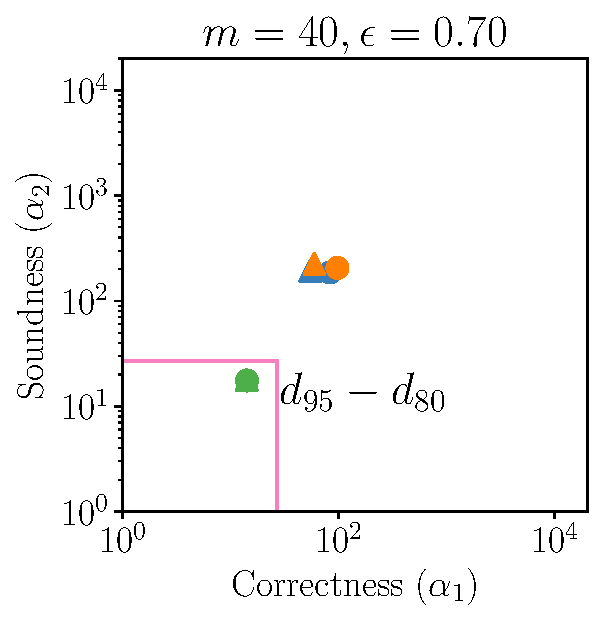
\includegraphics[width=0.23\linewidth]{Plots/gnm_def_40_0.7.pdf}
 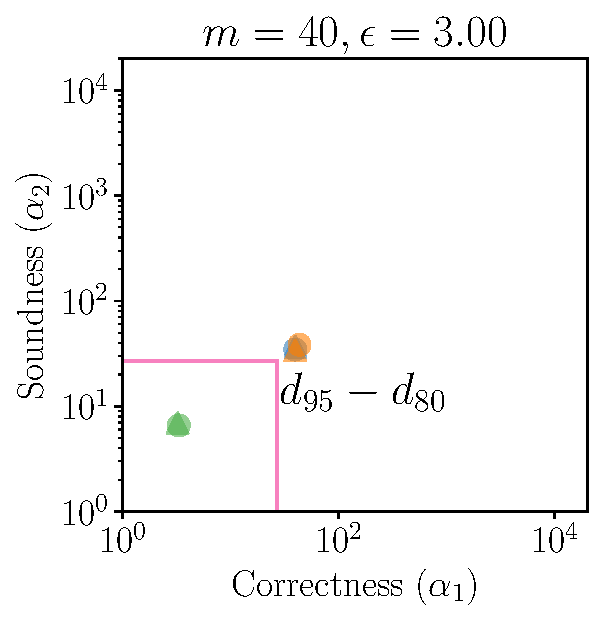
\includegraphics[width=0.23\linewidth]{Plots/gnm_def_40_3.0.pdf}
  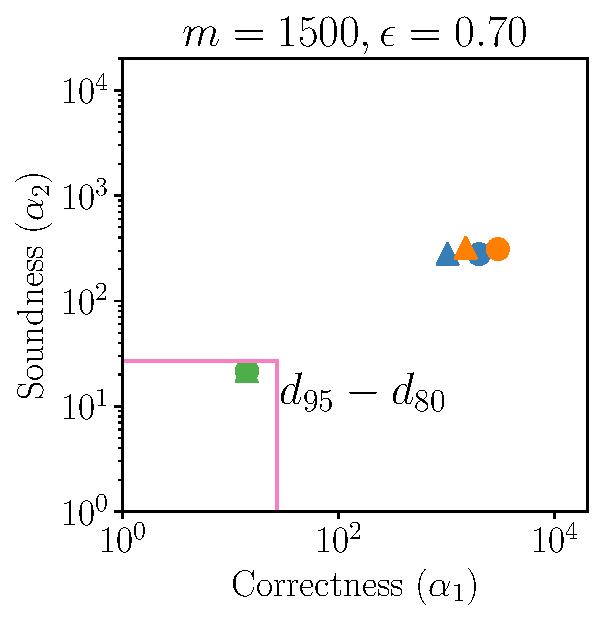
\includegraphics[width=0.23\linewidth]{Plots/gnm_def_1500_0.7.pdf}
 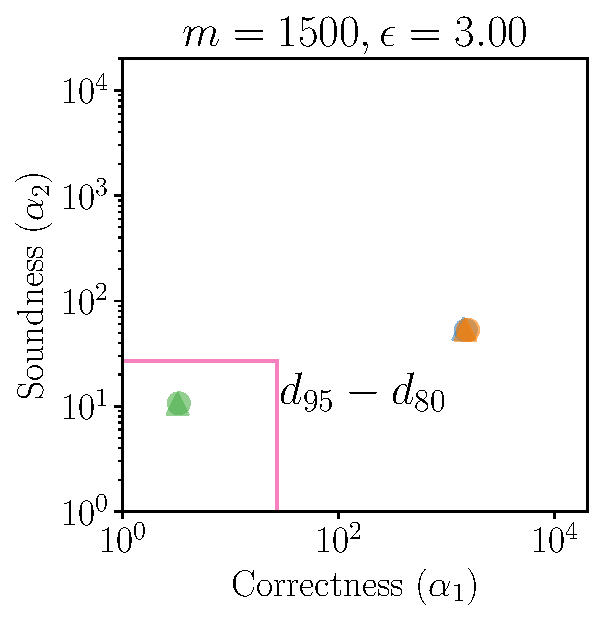
\includegraphics[width=0.23\linewidth]{Plots/gnm_def_1500_3.0.pdf}
  \vspace{-0.2cm}  \caption{\scalebox{0.8}{\textit{Syn}: Degree Deflation Attack}}
        \label{chap4-fig:Syn:defl}
        \end{subfigure}  \vspace{-0.5cm}  
\caption{Robustness Analysis for Degree Deflation Attack: We plot the empirical correctness (error of honest user) and soundness (error of malicious user). $d_{k}$ denotes the degree of the $k$ percentile node.}
\end{figure*}


\begin{figure}
  \begin{subfigure}[b]{0.49\linewidth}
    \centering 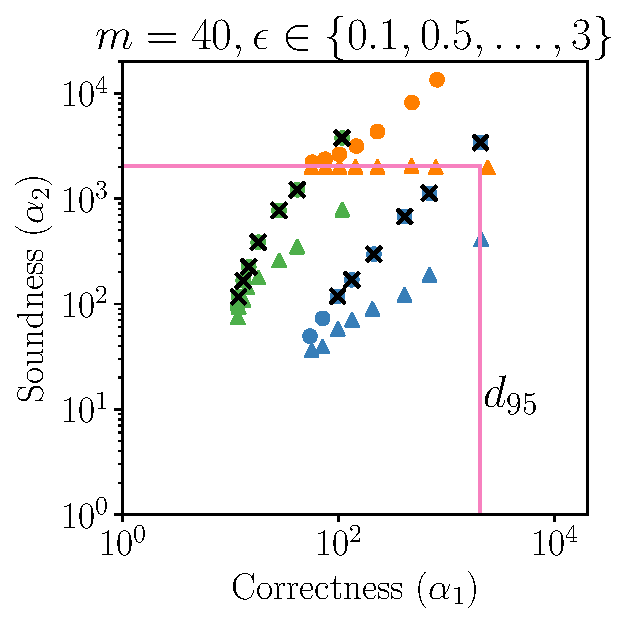
\includegraphics[width=1\linewidth]{Plots/gnm_inf_vary_40.pdf}  \vspace{-0.7cm}  
        \caption{\textit{Syn}: Degree Inflation Attack}
        \label{chap4-fig:Syn:privacy}\end{subfigure}
        \begin{subfigure}[b]{0.49\linewidth}
        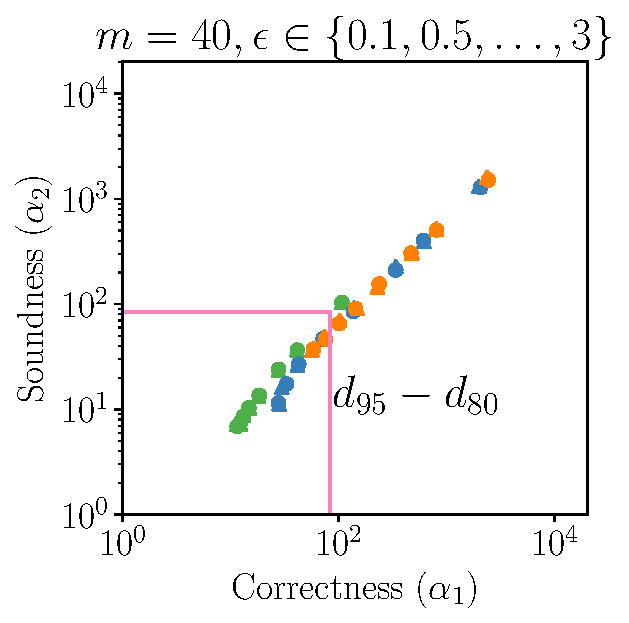
\includegraphics[width=\linewidth]{Plots/fb_def_vary_40.pdf}  \vspace{-0.7cm}  
        \caption{\textit{FB}: Degree Deflation Attack}
        \label{chap4-fig:FB:privacy}
        \end{subfigure}  \vspace{-0.3cm}  
\caption{Robustness analysis with varying $\epsilon$}
\end{figure}
\noindent \textbf{Protocols.} 
We evaluate our proposed \DegRRCheck{} and \DegHybrid{} protocols and use \DegRRNaive{} as a baseline protocol with poor robustness. %We ran each protocol on various graph datasets, with input and response poisoning attacks aimed at degree inflation and deflation, and with varying choices of parameters.
\vspace{-0.2cm}\\\\
\noindent\textbf{Attacks.} For each protocol, we evaluate two types of attacks -- degree inflation and degree deflation where the goal of the malicious users is to increase (resp. decrease) the degree estimate of a target malicious (resp. honest) user by as much as possible.
 We choose these attacks because firstly, they can meet the asymptotic theoretical error bounds.
%\footnote{Due to symmetry, attacks which target multiple users can be considered as a set of attacks with a single target. The only distinguishing feature is whether the targeted user is honest or malicious. Also due to symmetry, it is equivalent to consider either degree inflation or deflation attacks for one attacked target user, and the same for one target malicious user.}.
Secondly, these attacks are grounded in real-world motivations and represent practical threats (see Sec. \ref{chap4-sec:attacks}). For each attack type, we consider both input and response poisoning versions. In the following, let $\DO_t$ represent the target user. 
\vspace{-0.2cm}\\\\
\noindent\DegRRCheck{}. For the degree inflation attack, the non-target malicious users always report a $1$  for the malicious user $\DO_t$ (i.e. that they are connected to $\DO_t$) in the hopes of increasing $\DO_t$'s degree estimate.
Likewise, $\DO_t$ reports $1$s for all other malicious users. For the honest users, $\DO_t$ reports extra $1$s (for non-neighbors) in the hopes of further increasing their degree estimate. The exact mechanism depends on whether it is response poisoning or input poisoning and is detailed in App. \ref{chap4-app:attacks}.
\begin{comment}: For input poisoning, $\DO_t$ takes $q_1$ of their non-neighboring honest users and reports $1$. For response poisoning, $\DO_t$ simulates their true response by applying randomized response to his data, and then takes $q_1$ of the $0$s from that response and reports $1$s. During the trials, we used $q_1 = 15\%$, as at this threshold the chance of the $\DO_t$ being flagged as $\bottom$ became significant. For exact mechanisms for both input and response poisoning, see Appendix~\ref{chap4-app:attacks}.
\end{comment}

For degree deflation, we consider the worst-case scenario where $m$ of the neighbors of the honest user $\DO_t$ act maliciously. The malicious neighbors always report $0$ for their edges to $\DO_t$ (see App.~\ref{chap4-app:attacks}).
\vspace{-0.2cm}\\\\
\noindent\DegHybrid. %Recall that for this protocol, users report their edges via randomized response and a degree estimate $\tilde{d}_i^{lap}$ via the Laplace mechanism. 
For degree inflation, the non-target malicious users report their edges using the same strategy as in \DegRRCheck{}. For $\tilde{d}_i^{lap}$, they send their true degree estimates since their degrees are not the targets. Similarly, $\DO_t$ uses the same strategy as in $\DegRRCheck{}$ for reporting their edges. For $\tilde{d}_t^{lap}$, $\DO_t$  reports an inflated value based on the reported edges and the threshold $\tau$ (see  App. \ref{chap4-app:attacks}).

For degree deflation, we consider the worst-case scenario where $m$ of the neighbors of $\DO_t$ act maliciously. The malicious users behave as they did in \DegRRCheck{} and report their true degrees for $\tilde{d}_i^{lap}$, as these are not the targeted degrees.
\vspace{-0.2cm}\\\\
 \noindent\DegRRNaive. For degree inflation, we consider the worst-case scenario where the target malicious user $\DO_t$ is responsible reporting all their edges, and chooses to reports all $1$s. %For response poisoning, this is equivalent to Algorithm~\ref{chap4-alg:attack3}. For input poisoning, this is equivalent to running Algorithm~\ref{chap4-alg:attackinput} with all 1s as the poisoned input.

For degree deflation, we again consider the worst case scenario where the malicious users are responsible for reporting the edges to $\DO_t$, and they report $0$s.
\vspace{-0.2cm}\\\\
\noindent \textbf{Configuration.} %For each of the aforementioned graphs, we ran our three protocols against degree inflation and deflation attacks. 
 For degree inflation, we report the maximum error over all honest users (correctness, $\alpha_1$) and the error of the malicious target (soundness, $\alpha_2$). For degree deflation, we report the error of the honest target (correctness) and the maximum error over all the malicious users (soundness). We run each experiment $50$ times and report the mean.  We use $\delta=10^{-6}$ and $c = 0.9$ for \DegHybrid{}. Additional details are in App.~\ref{chap4-app:attacks}. %For each attack, we selected a random target user, and for degree inflation, we chose $m-1$ additional malicious users from the remaining nodes. For degree deflation, we selected a random target user and selected $m$ of that user's neighbors to be malicious. In degree inflation, we reported the error of the target's degree inflation (soundness) against the maximum error over all honest users (correctness). In degree deflation, we reported the maximum error of the malicious users' degrees (soundness) against the error of the target (correctness). %We performed both input and response versions of each attack type. We ran each attack version, including reselecting the target and malicious users, $50$ times and report the mean---if any user is flagged with $\bottom$, we simply report the mean over the smaller set. We use $\delta=10^{-8}$. .

\begin{comment}\begin{enumerate}\item Gap between theory and practice for degree vector \item Test other questions - \begin{itemize}\item degree histogram \item highest degree value \item highest degree node \end{itemize}\item Test adversary selection strategies \begin{itemize}\item adversaries belong to $k$-th percentile \item  target's degree \item malicious clients share an edge with the target vs do not share an edge \end{itemize}\end{enumerate}
\end{comment}
\vspace{-0.4cm}
\subsection{Results} \label{chap4-sec:exp-results}
%\arc{Report how many time the malicious user is caught for degree inflation}
 We consider two values of $m$ (number of malicious users): $m=40$ and $m=1500$. The former corresponds to $=1\%$ malicious users which represents a realistic threat model. We also consider $m=1500$ to showcase the efficacy of our protocols even with a large number of malicious users ($=37.5\%$).
\vspace{-0.2cm}\\\\\noindent\textit{Degree Inflation.} We report our results for degree inflation in Figs.~\ref{chap4-fig:FB:infl} and~\ref{chap4-fig:syn:infl}.  In terms of correctness, we observe that \DegHybrid{} performs the best --- this is expected since the error introduced by the Laplace mechanism of $\tilde{O}(\frac{1}{\epsilon})$ is the lowest. Both \DegRRCheck{} and \DegRRNaive{}  have higher honest error of $\tilde{O}(\frac{\sqrt{n}}{\epsilon})$ due to the underlying randomized response mechanisms. \DegRRCheck{} has better correctness than \DegRRNaive{}, particularly for \textit{FB} with low privacy ($\epsilon=3$). This is because the degree estimator for \DegRRNaive{} is based on the random variable $count^{1}$  (Sec. \ref{chap4-sec:protocol:naive}) which  has a variance $n\rho(1-\rho)$. However, the degree estimator for \DegRRCheck{} is based on the random variable $count^{11}$ (Sec. \ref{chap4-sec:protocol:check}). The variance of $count^{11}$ is a function of the graph degree distribution and is lower than that of $count^{1}$ for sparse graphs and high $\epsilon$. 
In terms of soundness, both our proposed protocols perform better than the baseline  -- \DegRRNaive{}  has $43\times$ and $60\times$ higher malicious error than \DegHybrid{} and \DegRRCheck, respectively, for \textit{FB} for $\epsilon=3, m=40$ for input poisoning. Note that \DegRRCheck{} performs slightly better than \DegHybrid. This is because, although both the protocols have the same asymptotic soundness guarantee, the constants are higher for \DegHybrid (see Sec. \ref{chap4-sec:hybrid}). %This is because the additional Laplace degree estimate gives an extra way for the malicious target to cheat, as described in the attacks section. However, as noted in Section~\ref{chap4-sec:hybrid:attack}, this difference is only up to constants, the asymptotic soundness guarantee of \DegRRCheck{} and \DegHybrid{} is the same. 
Finally, we observe that response poisoning is worse than input poisoning for all the protocols for soundness, which is to be expected and is consistent with the theory (response poisoning has an extra $O(\frac{m}{\epsilon}$) term). For instance, for \DegRRCheck{}, response poisoning is $4.2\times$ worse than input poisoning for \textit{Syn} with $m=1500,\epsilon=0.7$. As expected, the separation becomes less prominent with higher privacy and lower $m$, as it is harder to pull off strong attacks for these regimes.



\par Figs. \ref{chap4-fig:FB:infl} and \ref{chap4-fig:syn:infl} also mark the degree of $95^{th}$ percentile node ($d_{95}$) for the respective graphs. The way to interpret this is as follows.  If an error of a protocol falls outside the box, then any malicious user can inflate their degree estimate to be in the $>d_{95}$ percentile by staging a poisoning attack. Our protocols are better performant for the dense graph \textit{Syn} (attacks are prevented for both values of $\epsilon$). This is because of the $\tilde{O}(\frac{\sqrt{n}}{\epsilon})$ term in the soundness guarantee -- this term dominates the malicious error for sparse graphs. 

\par Finally, for both datasets for $m=40$ and $\epsilon = 0.7$, our protocols flag the malicious target user (returning $\bottom$) for $30\%-70\%$ of the trials.  We indicate this with an ``X'' in the figures. This indicates that our proposed protocols are able to detect malicious users, thereby disincentivizing malicious activity.
\vspace{-0.2cm}\\\\
\noindent\textbf{Degree Deflation.}
Figs. \ref{chap4-fig:FB:defl} and  \ref{chap4-fig:Syn:defl} show the results for the degree deflation attacks on  \textit{FB} and \textit{Syn}, respectively. We observe that \DegHybrid{} performs the best in terms of both correctness and soundness. For instance, it has $58\times$ and $20\times$ better correctness than \DegRRNaive{} and \DegRRCheck{}, respectively, for \textit{FB} and response poisoning with $\epsilon=0.7, m=1500$. $\DegRRCheck{}$ and $\DegRRNaive{}$ have similar correctness. This is because the correctness guarantees for both protocols are asymptotically the same. %The correctness of $\DegRRCheck{}$ is between that of $\DegHybrid{}$ and $\DegRRNaive{}$, and it is better than $\DegRRNaive{}$ by small factors between $1-2$. This is consistent with the theoretical results, as the correctness guarantees for both protocols are asymptotically the same.
The soundness error for these two protocols are from just the underlying randomized response mechanisms. We observe that \DegRRCheck{} has better soundness than  \DegRRNaive{} for \textit{FB} for $\epsilon=3$ because of a better degree estimator as described previously. Finally, we observe that the response poisoning is more damaging than input poisoning for \DegRRNaive{} and \DegRRCheck. For instance, response poisoning has $2\times$ worse correctness than input poisoning for \DegRRCheck{} for \textit{Syn} with $\epsilon=0.7,m=1500$. However, the two types of poisoning have a similar impact on the correctness of \DegHybrid{}, as the final degree estimate sent by the target user via the estimate from the Laplace mechanism is not poisoned.

We note that none of the degree deflation attacks resulted in the honest user being falsely flagged, demonstrating empirically  that our protocols do not have false positives.

We plot the measure $d_{95}-d_{80}$ in Figs. \ref{chap4-fig:FB:defl} and \ref{chap4-fig:Syn:defl} where $d_{k}$ denotes the degree of the $k$ percentile node. The way to interpret this is as follows. If an error falls outside the box, then malicious users can successfully deflate the degree of an honest target from $>95$ percentile to $<80$ percentile. Based on our results, we observe that \DegHybrid{} is mostly effective in protecting against this attack even with a large number of malicious users of $m=1500$. 
 %Additionally, 
%We make similar observations for the \textit{Syn} dataset (Fig. \ref{chap4-fig:Syn}) on all four attacks. The only distinction here is that, since \textit{Syn} is a dense graph, the relative error of \DegRRCheck$(\cdot)$ is significantly smaller than that for the sparse \textit{FB} graph. Hence, it might be acceptable to use \DegRRCheck$(\cdot)$ for dense graphs  especially for degree inflation type attacks.
\vspace{-0.2cm}\\\\
\noindent\textbf{The effect of $\epsilon$.} Figs. \ref{chap4-fig:FB:privacy} and \ref{chap4-fig:Syn:privacy} show the impact of the attacks with varying privacy parameter $\epsilon$. We observe that, increasing privacy (lower $\epsilon$) leads to more skew for all attacks on all three protocols. For instance, the response poisoning version of the degree deflation attack for \textit{FB}  is $74\times$ worse for $\epsilon=0.1$ than that for $\epsilon=3$ for \DegRRCheck{}. Additionally, we observe that malicious users get flagged only for input poisoning for larger $\epsilon$. This is because for small values of $\epsilon$, the thresholds are large due to more noise introduced by privacy which makes it harder to detect malicious users. 
\par Another interesting observation is that even a relatively small number of malicious parties ($m=1\%$) can stage significantly damaging poisoning attacks. This demonstrates the practical threat of such poisoning attacks. As expected, the impact of the poisoning attacks worsens with increasing $m$. Nevertheless, our results show that our proposed protocols are able to significantly reduce the impact of poisoning attacks even with a large number of malicious users ($m=37.5\%$).
%\arc{Input error higher than response \\Malicious error should be higher than honest error}
%This is a realistic assumption in many scenarios. Next, we considered a highly adversarial $1500$ adversaries. While many of the protocols do not perform well for this setting, this setting illustrates several important concepts for our protocol.

 %Our low value of $\epsilon$ is a strong privacy guarantee and serves to highlight the increased susceptibility of the protocols to attacks. Our higher value of $\epsilon$ is more in line with values typically used in practice.


\begin{comment}
\arc{Jotting down the main observations, their possible explanations and current anomalies (A) in the graph}
95th percentile gain not really --
Degree Inflation: FB
\begin{itemize}
\item No attack on honest users
    \item Response > Input for all settings, more prominent for low eps, high m - A: 5a.2 (sqrt{n}{eps} dominates) , 5a.2 Why is inout and response flipped for RRcheck? 5a. 4 -- sqrt{n}{eps} dominating despite high m?
    \item Why is the honest error increasing for RRcheck with high m - it should not be affected at all?
    \item Error for Naive does not increase because of our protocol - target had control over all edges 
    \item Hybrid has lowest honest error
    \item RRcheck has lower malicious error than Hybrid - order same, higher constants
    \item Honest error for Naive < for RRcheck - better estimator -A: M=40 and M=1500 contradictory
\end{itemize}

Degree Deflation: FB
\begin{itemize}
    \item Needs new deflation attack for RRNaive
    \item No malicious error
    \item A: Why is the difference between the response and input not prominent here even for low eps high m - acceptable for Hybrid?
    \item Honest/malicious error does not change with m for Hybrid
    \item A: Malicious error increases for RRcheck with m- why, honest error should increase more for RRcheck?
    
\end{itemize}

For Syn
\begin{itemize}
    \item A: what is the gain of RRcheck now is not clear
    \item A: M=1500 seems to be exactly the same as that of FB
\end{itemize}



In Figure~\ref{chap4-fig:my_label}, we plot the malicious error and honest error as a point for the \textit{FB} graph, for both degree inflation and degree deflation attacks, for two values of $m$ and $\epsilon$. Around each point, we also plotted an ellipse of radius $3$ times the sample standard deviations, indicating a $99\%$ chance that the true values lie within the ellipse. Note the ellipses are distorted due to the log axis. Often, the ellipse is smaller than the point and is not visible. We have the following findings.

First, it is often true that $\DegHybrid{}$ performs better than the other two protocols in terms of both honest and malicious error. The honest error is about $5$ to $10$ times better than the other two algorithms, and is never worse than about $40$ (for $\epsilon = 0.3$) and about $10$ (for $\epsilon = 3.1$). \arc{from Fig 5, the honest error of \DegHybrid~is never worse than the other two (as it should be) - why do you say "never worse than about $40$ (for $\epsilon = 0.3$) and about $10$ (for $\epsilon = 3.1$)" this then?} The other two algorithms have honest error of at least $600$ and $25$, respectively. For malicious error, a similar observation holds for the degree deflation attacks. However, for the degree inflation attacks, $\DegRRCheck{}$ outperforms $\DegHybrid$ by a factor of $2$ to $5$. For example, when $\epsilon = 3.1$ and $m=40$, the malicious error for response poisoning is $195$ for \DegHybrid{} and $35$ for \DegRRCheck{}. \arc{they are order optimal but \DegHybrid~has higher concrete constants due to the second check}

In comparing \DegRRCheck{} with \DegRRNaive{}, the former algorithm attains less honest error than the latter for $40$ adversaries by a factor of $1$ to $2$. \ji{Why is this true?}. However, for $1500$ adversaries, the \DegRRNaive{} attains less honest error by a factor of at least $5$. \DegRRCheck{} always attains less malicious error than \DegRRNaive{}, and for the degree inflation attacks, it obtains the best malicious error of $35, 82$ for response and input poisoning attacks for $\epsilon = 3.1$ on $40$ adversaries.

Second, in general the degree inflation attacks are effective at $\epsilon = 0.3$, where an adversary is able to add at least a few hundred to his degree. However, at $\epsilon = 3.1$, \DegRRCheck{} is resistant to poisoning, attaining honest error no more than $26$ and malicious error no more than $82$.
For degree deflation attacks, $\DegHybrid{}$ attains errors less than $40$ (resp. $10$) for $\epsilon = 0.3, 3.1$ at all numbers of adversaries.

Third, for degree inflation, input poisoning is generally a less effective than response poisoning, particularly at lower levels of privacy. For example, with $40$ adversaries, the malicious error inflicted on \DegHybrid{} is $1200, 2700$ for input and response poisoning, respectively. This ratio for the other mechanisms is even larger. However, for $\epsilon = 3.1$, the malicious errors of input and response poisoning converge, with less than a $5\%$ difference.
For degree deflation, there is no noticeable gap between input poisoning and response poisoning, except for \DegRRCheck{} when $\epsilon = 0.3$: there, input poisoning attains honest error of $1250$ while response poisoning attains honest error of $2530$.
\ji{Check why the input poisoning error is sometimes higher than the response poisoning error for the FB graph.}

\end{comment}

  \vspace{-0.4cm}  \subsection{Discussion}\label{chap4-sec:exp-discuss}
Here, we discuss our empirical results in the context of our three evaluation questions. First, we observe that the baseline protocol \DegRRNaive{}  performs worse than both our proposed protocols. \DegHybrid{} offers the best correctness guarantee and its soundness is at least comparable to that of \DegRRCheck{} for all the attacks. Concretely, \DegHybrid{} can improve the correctness  and soundness by up to $25\times$  and $58\times$, respectively, as compared to that for \DegRRNaive. Second, we observe that the response poisoning is stronger than input poisoning for all four attacks and all three protocols. Concretely, the response poisoning can be up to $4.2\times$ worse than input poisoning.
Finally, we see that the privacy exacerbates the impact of the poisoning attacks -- both correctness and soundness gets worse with lower values of $\epsilon$ for all attacks on all three protocols. Concretely, poisoning can worsen by up to $74\times$ for a drop in privacy from $\epsilon=3$ to $\epsilon=0.7$.